% Created 2021-06-21 Mon 10:34
% Intended LaTeX compiler: pdflatex
\documentclass[11pt]{article}
\usepackage[utf8]{inputenc}
\usepackage[T1]{fontenc}
\usepackage{graphicx}
\usepackage{grffile}
\usepackage{longtable}
\usepackage{wrapfig}
\usepackage{rotating}
\usepackage[normalem]{ulem}
\usepackage{amsmath}
\usepackage{textcomp}
\usepackage{amssymb}
\usepackage{capt-of}
\usepackage{hyperref}
\author{chris hepplewhite}
\date{\today}
\title{}
\hypersetup{
 pdfauthor={chris hepplewhite},
 pdftitle={},
 pdfkeywords={},
 pdfsubject={},
 pdfcreator={Emacs 26.3 (Org mode 9.1)}, 
 pdflang={English}}
\begin{document}

\tableofcontents

\begin{titlepage}
 
This is the title page

\end{titlepage}


\section{Purpose and Scope}
\label{sec:org143a6d7}

The purpose of the work reported herein is to qualify that the CHIRP product as supplied
by the DAAC conforms to the same as designed by the group at UMBC/JCET.

The CHIRP product is currently derived from three parent sensor records; the NASA Aqua AIRS; the
NOAA SNPP CrIS, and the NOAA JPSS-1 CrIS. In each case the original radiance spectra are 
translated to the CHIRP spectral grid, and the geolocation data are copied forward to the
CHIRP data, such that the format and content of each granule of the parent matches the granule
of the CHIRP.

The scope of this work includes verification that the translation of the radiance to the
CHIRP spectral grid conforms to that prescribed by the concurrent version of translation
suite established at UMBC/JCET. In addition, that the granule geolocation data are unchanged
from the parent sensor record.

The intent here is only to qualify that the spectral translation and bias shift have been
applied correctly to the parent spectra, and that the geolocation of the parent granule
is unchanged by the processing.


\section{Experiments}
\label{sec:org592b646}

A single experiment is conducted on each of the three CHIRP products. This involved
selecting a granule with some views of warm ocean and cold clouds and comparing geolocation
and radiance data from the CHIRP and the parent sensor record for the same granule.
A different granule is required for the three versions, but all are chosen from 
01-Jan-2020.

The radiance data from the parent sensor for the chosen granule is passed through the
translation code and compared to those from the CHIRP granule. There are typically 12150
observations per granule. The values are simply compared as shown in the following figures.

\section{Results}
\label{sec:org8adc8c9}

The results are shown in graphical form in the following figures. 
Figures show the location of the granule, with the LW window channel near 900 \(cm^{-1}\) 
brightness temperature.
Also the individual sample geolocation compared between the CHIRP and the parent granule
and a LW window channel signal difference for every sample in the granule.
Finally the spectrum of the granule mean and standard deviation of the samples and
the difference between CHIRP and parent product. 

\subsection{CHIRP.J1}
\label{sec:org46d2734}

This set of results relates to the CHIRP from JPSS-1 and its parent.

Figure Fig. \ref{fig:chirp_j1_map} shows the 900 cm-1 brightnes temperature for the selected granule, being in the tropical pacific Ocean.

Figure Fig. \ref{fig:chirp_j1_geo} shows the differences of the time, the latitude and the longitude of every sample in the granule  reported in the CHIRP and the parent granule. The difference of the 899.375 cm-1 channel BT is also shown. there is no difference in the geolocation data and only single bit differences in the BT, which are negligible.

Figure Fig. \ref{fig:chirp_j1_spectrum_mean} upper panel shows the mean BT spectrum for all samples in the granule for the CHIRP and parent. The lower panel shows the difference of the means, which is negligible in all CHIRP channels.

Figure Fig. \ref{fig:chirp_j1_spectrum_std} upper panel shows the standard deviation of the samples in the granule for both the CHIRP and its parent, and the lower panel the difference of the sample standard deviations. Again there is negligible difference.

\begin{figure}[htbp]
\centering
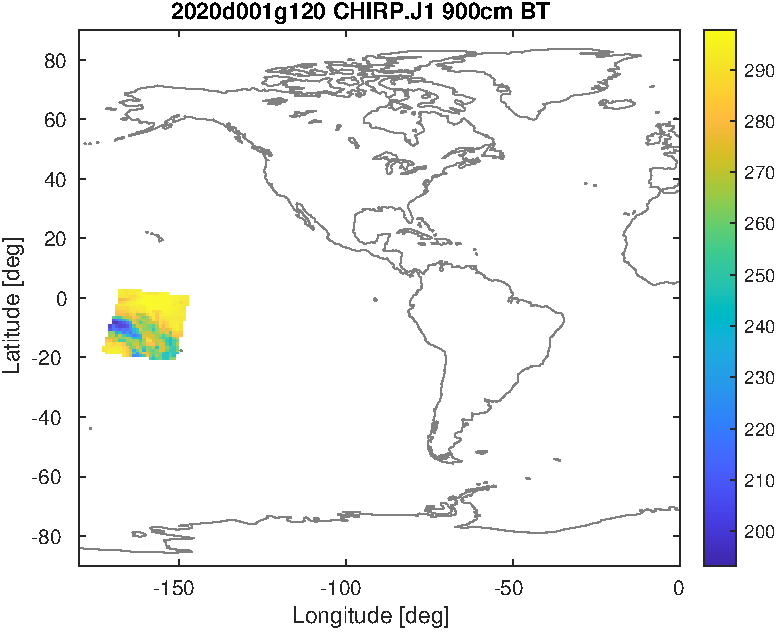
\includegraphics[angle=0,width=9cm]{./figs/2020d001g120_chirp_j1_900cn_bt_map.pdf}
\caption{\label{fig:orgca42ef6}
Location map of test granule. Shown is the 900cm-1 channel brightness temperature.}
\end{figure}

\begin{figure}[htbp]
\centering
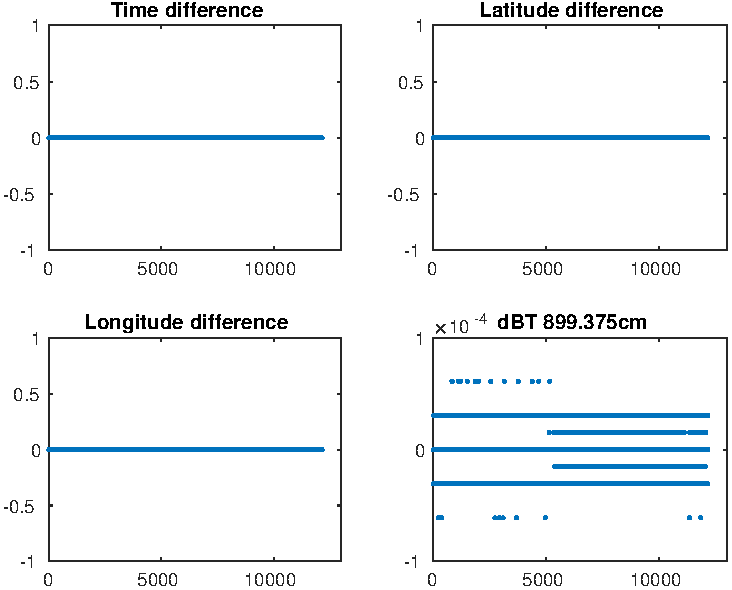
\includegraphics[width=.9\linewidth]{./figs/2020d001g120_chirp_j1_geo_diff.pdf}
\caption{\label{fig:orgfa70246}
Geolocation (latitude, longitude, time) difference by sample in granule. LW channel difference.}
\end{figure}

\begin{figure}[htbp]
\centering
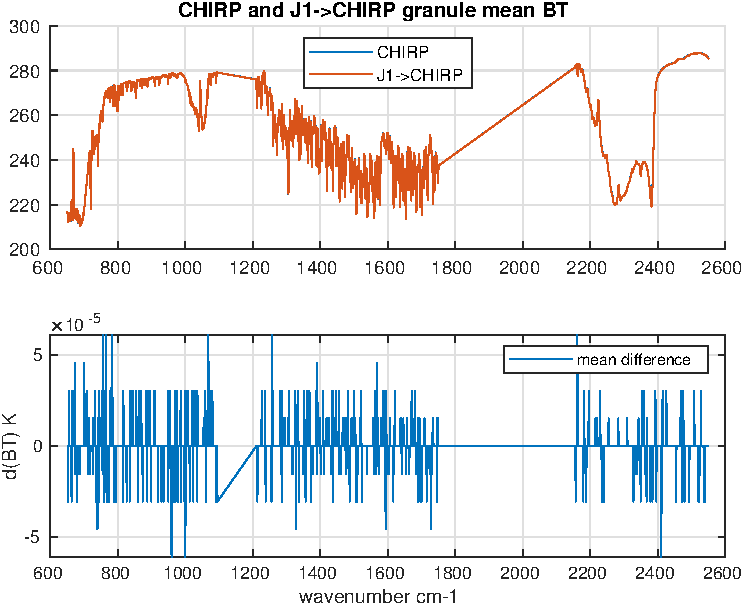
\includegraphics[width=.9\linewidth]{./figs/2020d001g120_chirp_j1_bt_spectrum_mean.pdf}
\caption{\label{fig:org7a964df}
Mean spectral BT for granule (upper) Difference (lower).}
\end{figure}

\begin{figure}[htbp]
\centering
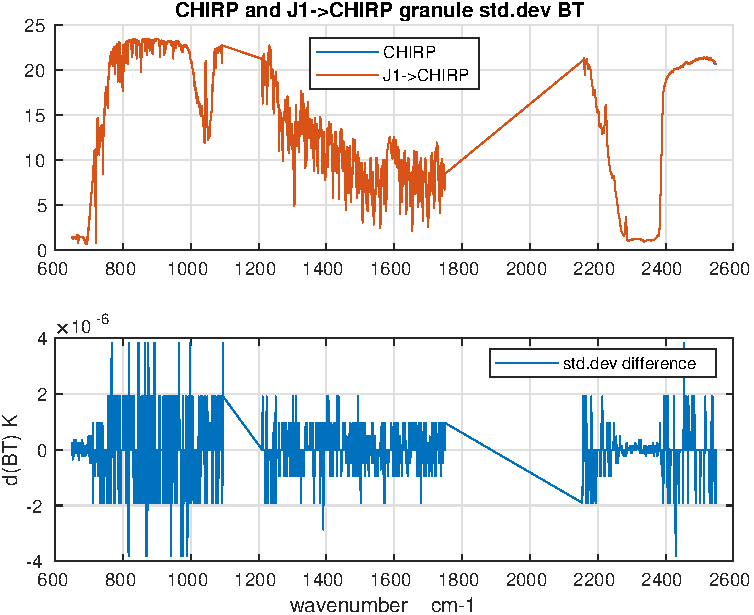
\includegraphics[width=.9\linewidth]{./figs/2020d001g120_chirp_j1_bt_spectrum_std.pdf}
\caption{\label{fig:org44ee57e}
Standard deviation of samples (upper) Difference (lower).}
\end{figure}




\subsection{CHIRP.SNPP}
\label{sec:orgd452a14}

This set of results relates to the CHIRP from SNPP and its parent.

Figure Fig. \ref{fig:chirp_snpp_map} shows the 900 cm-1 brightnes temperature for the selected granule, being in the tropical pacific Ocean.

Figure Fig. \ref{fig:chirp_snpp_geo} shows the differences of the time, the latitude and the longitude of every sample in the granule  reported in the CHIRP and the parent granule. The difference of the 899.375 cm-1 channel BT is also shown. there is no difference in the geolocation data and BT.

Figure Fig. \ref{fig:chirp_snpp_spectrum_mean} upper panel shows the mean BT spectrum for all samples in the granule for the CHIRP and parent. The lower panel shows the difference of the means, which is effectively zero in all CHIRP channels.

Figure Fig. \ref{fig:chirp_snpp_spectrum_std} upper panel shows the standard deviation of the samples in the granule for both the CHIRP and its parent, and the lower panel the difference of the sample standard deviations. Again there is no difference.

\begin{figure}[htbp]
\centering
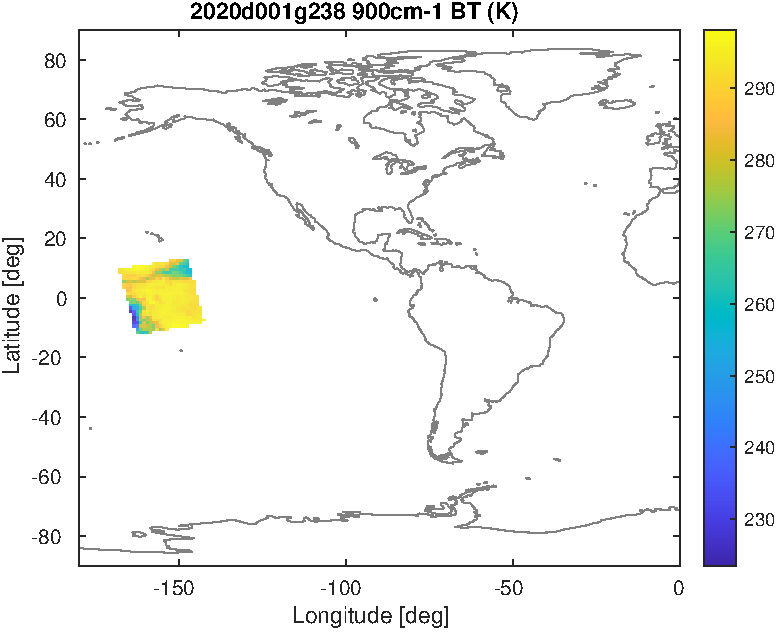
\includegraphics[angle=0,width=9cm]{./figs/2020d001g238_900cm_bt_map_snpp.pdf}
\caption{\label{fig:org1ad1365}
Location map of test granule. Shown is the 900cm-1 channel brightness temperature.}
\end{figure}

\begin{figure}[htbp]
\centering
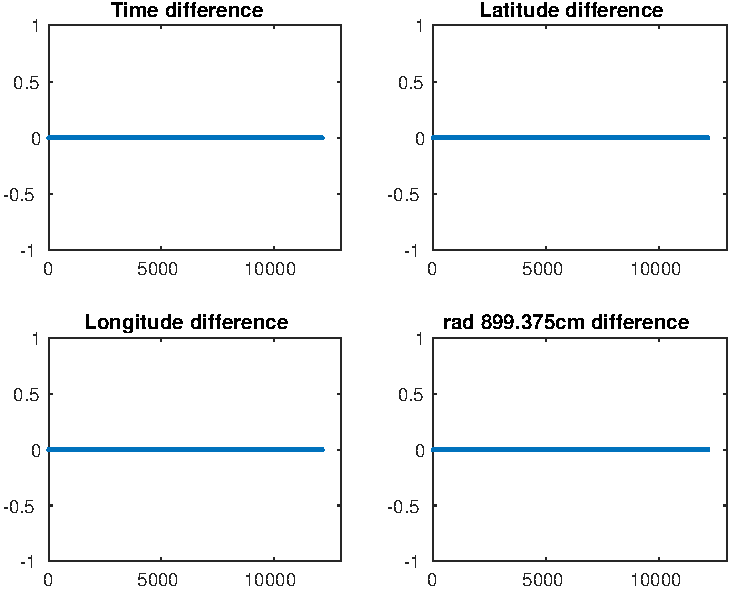
\includegraphics[width=.9\linewidth]{./figs/2020d001g238_geo_diff_snpp.pdf}
\caption{\label{fig:org6431cfd}
Geolocation (latitude, longitude, time) difference by sample in granule. LW channel difference.}
\end{figure}

\begin{figure}[htbp]
\centering
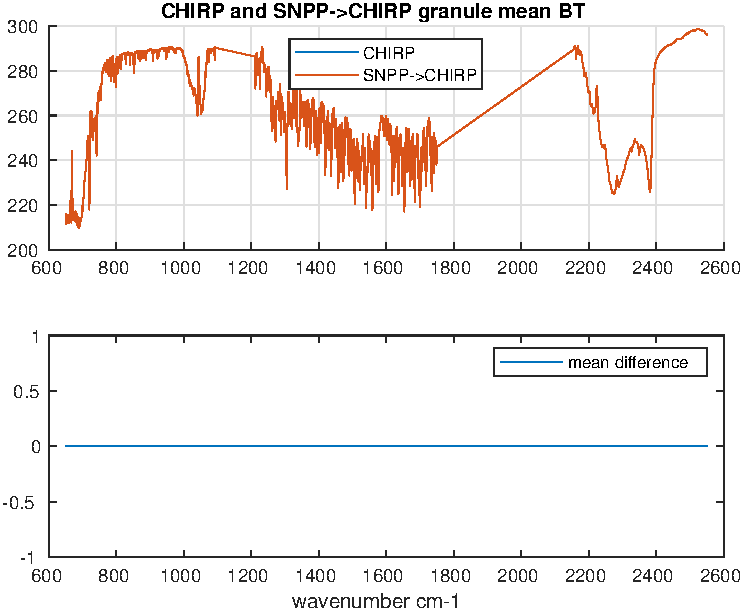
\includegraphics[width=.9\linewidth]{./figs/2020d001g238_bt_spectrum_mean.pdf}
\caption{\label{fig:org307d829}
Mean spectral BT for granule (upper) Difference (lower).}
\end{figure}

\begin{figure}[htbp]
\centering
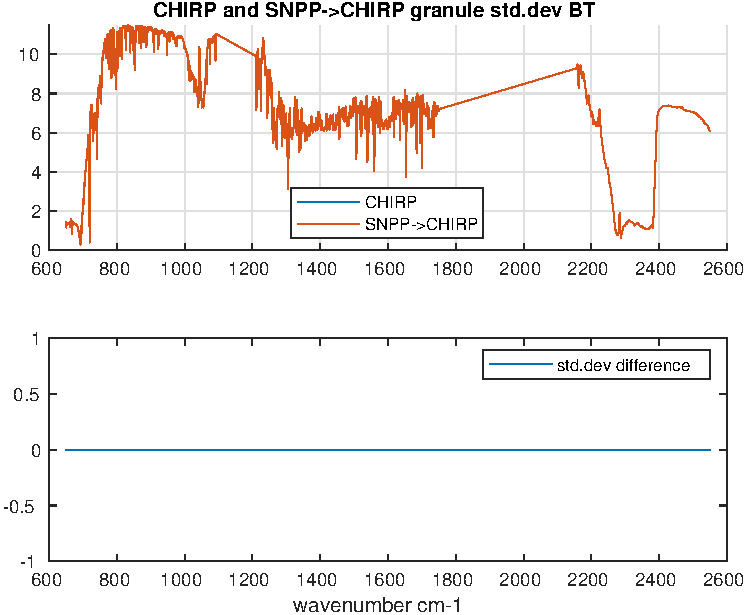
\includegraphics[width=.9\linewidth]{./figs/2020d001g238_bt_spectrum_std.pdf}
\caption{\label{fig:org084790a}
Standard deviation of samples (upper) Difference (lower).}
\end{figure}



\subsection{CHIRP.AQ}
\label{sec:orgdc9dda5}

This set of results relates to the CHIRP from AIRS and its parent.

Figure Fig. \ref{fig:chirp_aq_map} shows the 900 cm-1 brightnes temperature for the selected granule, being in the tropical pacific Ocean.

Figure Fig. \ref{fig:chirp_aq_geo} shows the differences of the time, the latitude and the longitude of every sample in the granule  reported in the CHIRP and the parent granule. The difference of the 899.375 cm-1 channel BT is also shown. The differences in the geolocation data are negligible and can be ignored, the difference in the 893.375 cm-1 BT channel are typically seen as the conversion routine does most work for AIRS, and the difference is negligible.

Figure Fig. \ref{fig:chirp_aq_spectrum_mean} upper panel shows the mean BT spectrum for all samples in the granule for the CHIRP and parent. The lower panel shows the difference of the means, which is very small and centered on zero in all CHIRP channels and is effectively negligible.

Figure Fig. \ref{fig:chirp_aq_spectrum_std} upper panel shows the standard deviation of the samples in the granule for both the CHIRP and its parent, and the lower panel the difference of the sample standard deviations. The differences are very small and centered on zero in all channels and is effectively negligible.

\begin{figure}[htbp]
\centering
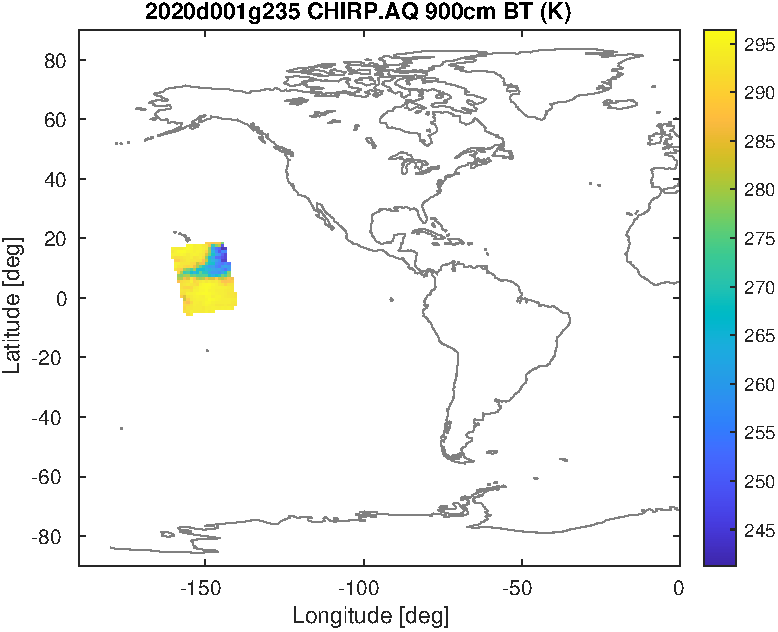
\includegraphics[angle=0,width=9cm]{./figs/2020d001g235_chirp_aq_900cm_bt_map.pdf}
\caption{\label{fig:orgd919374}
Location map of test granule. Shown is the 900cm-1 channel brightness temperature.}
\end{figure}

\begin{figure}[htbp]
\centering
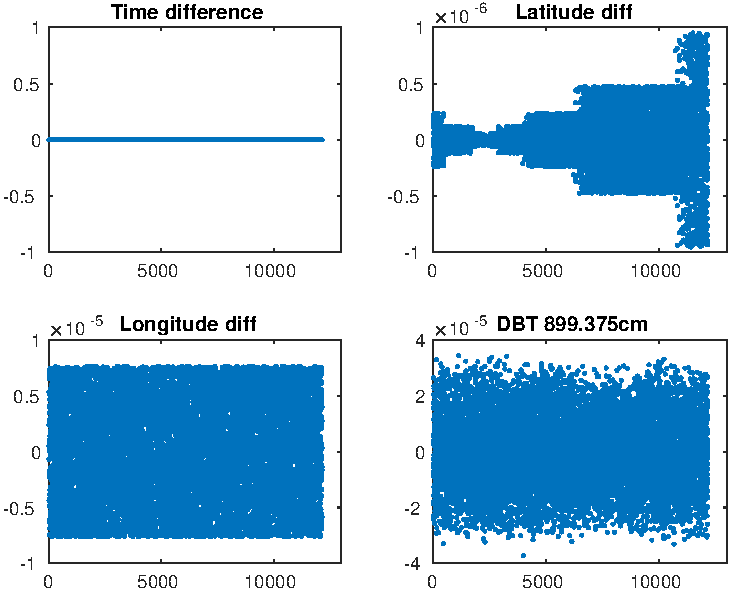
\includegraphics[width=.9\linewidth]{./figs/2020d001g235_chirp_aq_geo_diff.pdf}
\caption{\label{fig:org7d36680}
Geolocation (latitude, longitude, time) difference by sample in granule. LW channel difference.}
\end{figure}

\begin{figure}[htbp]
\centering
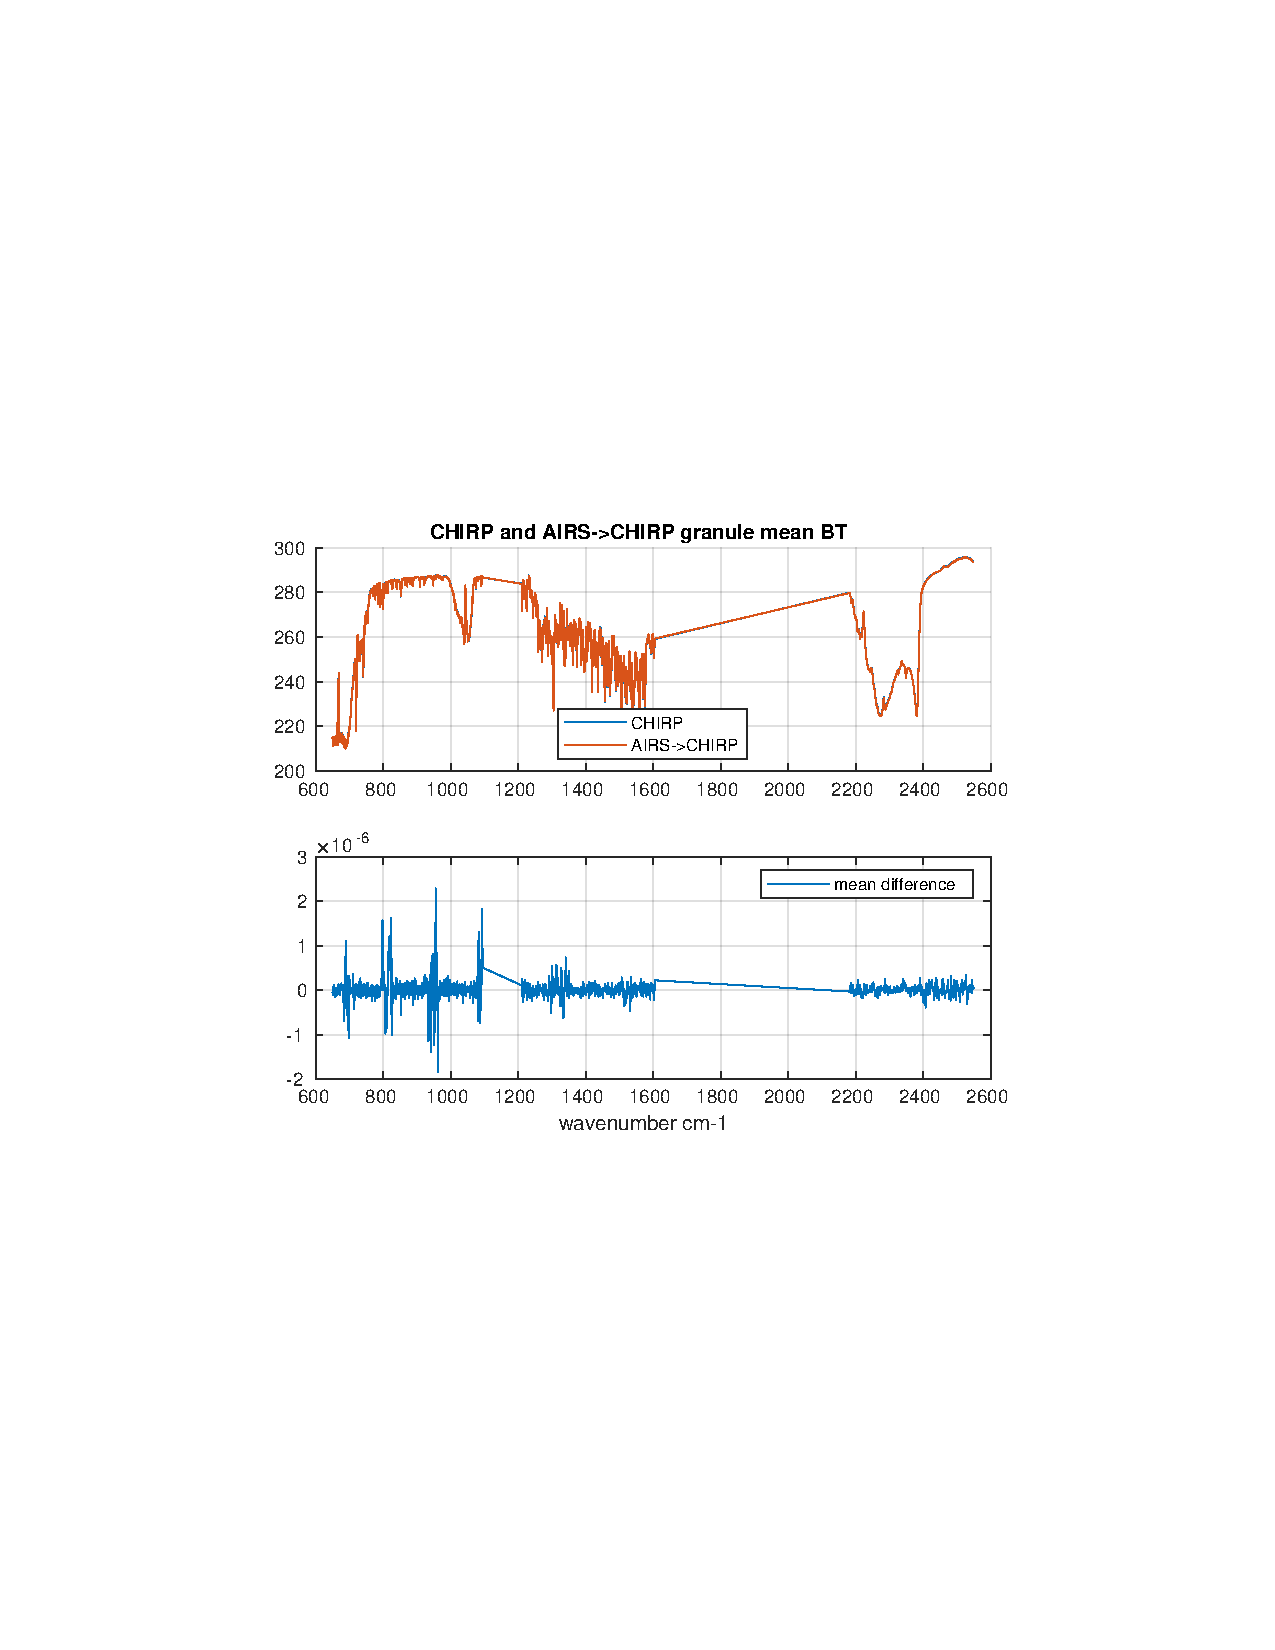
\includegraphics[width=.9\linewidth]{./figs/2020d001g235_chirp_aq_bt_spectrum_mean.pdf}
\caption{\label{fig:orgc712f95}
Mean spectral BT for granule (upper) Difference (lower).}
\end{figure}

\begin{figure}[htbp]
\centering
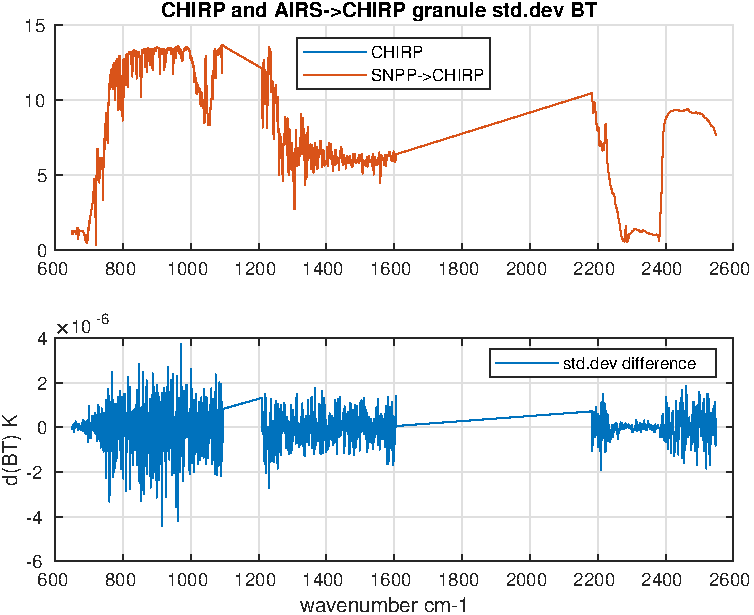
\includegraphics[width=.9\linewidth]{./figs/2020d001g235_chirp_aq_bt_spectrum_std.pdf}
\caption{\label{fig:org8647f29}
Standard deviation of samples (upper) Difference (lower).}
\end{figure}


\section{Conclusions}
\label{sec:org3c42b5a}
\end{document}
